\section{Full-Adder}
\subsection{Introduction}%Purpose, brief intro, Contribution 
    \subsubsection{Background}%What is the full adder, the key differences between the half adder and full adder, et cetera.
    The full adder is the basic component in digital circuits to carry out
    arithmetic operations. Different from the half adder, the full adder
    handles the addition of three inputs(A, B, and Carry-in) and output 
    the sum and carry-out of them.

    \subsubsection{Purpose}
    In this experiment, we want to design a full adder using the FPGA board that can handle three single-bit input additions. 

    \subsubsection{Design and Key-results}
    
\subsection{Materials and Methods}%Show FPGA solution
    \subsubsection{Structure Block Diagram}
        \begin{figure}[h]
        \centering
        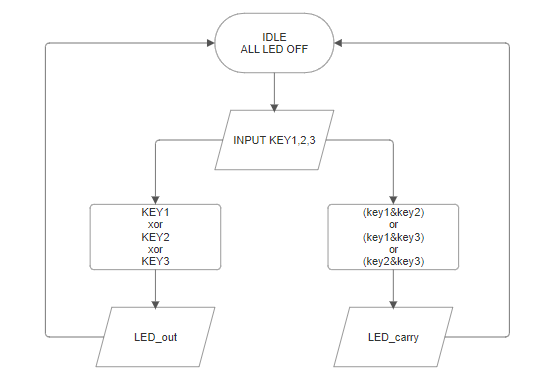
\includegraphics[width=0.8\linewidth]{Structure_Block_Diagram/fulladder_BlockStructureDiagram.png}
        \label{fa_SBD}
    \end{figure}
    \FloatBarrier
    \subsubsection{Truth Table}
    \begin{table}[h]
    \centering
        \begin{tabular}{|c|c|c|c|c|}
        \hline
        Key1 & Key2 & Key3 & LED\textunderscore cout & LED\textunderscore out \\ \hline
        0 & 0 & 0 & 0 & 0 \\ \hline
        0 & 0 & 1 & 0 & 1 \\ \hline
        0 & 1 & 0 & 0 & 1 \\ \hline
        0 & 1 & 1 & 1 & 0 \\ \hline
        1 & 0 & 0 & 0 & 1 \\ \hline
        1 & 0 & 1 & 1 & 0 \\ \hline
        1 & 1 & 0 & 1 & 0 \\ \hline
        1 & 1 & 1 & 1 & 1 \\ \hline
        \end{tabular}
    \end{table}
    \FloatBarrier
    \subsubsection{Signal Waveforms}
    \begin{figure}[h]
        \centering
        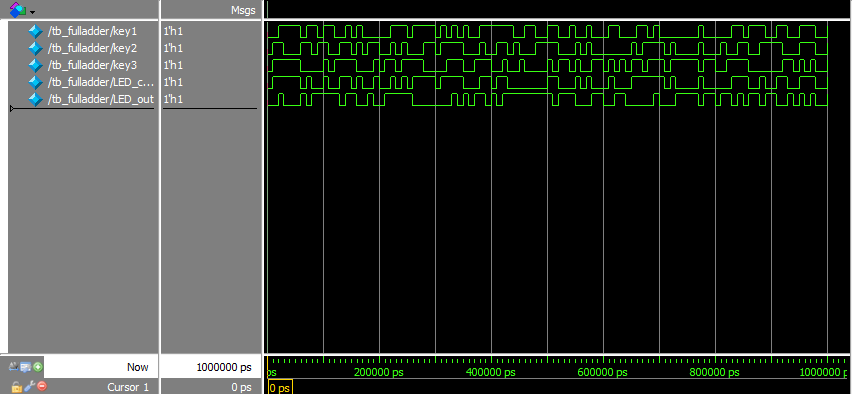
\includegraphics[width=0.8\linewidth]{Testbench_Waveform/tb_fulladder_waveform.png}
        \label{tb_fa}
    \end{figure}
    \FloatBarrier
    \subsubsection{Resources in Board}

\subsection{Results}%Show simulation and corresponding test results
    \subsubsection{Testbench}
    In this experiment, the testbench was built to accept three one-bit inputs. The testing inputs were randomly generated, and the outputs were presented by waveform. The expected results are listed below (carry, out):
    \begin{enumerate}
        \item All inputs are 0s. Output 0,0
        \item One input is 1, and two are 0s. Output 0,1
        \item Two inputs are 1, and one is 0. Output 1,0
        \item ALL inputs are 1s. Output 1,1
    \end{enumerate}
    It turned out that the actual output value was the same as we predicted.

\subsection{Discussions and Conclusion}
    \subsubsection{Discussions}%This is an optional bonus part, it is not essential.
    We encountered the problem of the testbench simulation not giving out the waveform plot in this experiment. It turns out that it is the problem with the testbench codes, in which the initiation part has the wrong name.
    \subsubsection{Conclusion}
    In this experiment, we learned how to use Quartus to create an FPGA project, write a Verilog code, and develop a testbench for the Verilog design.
\subsection{Appendices} References and Appendices
    \subsubsection{Reference}%This is a list of all the sources cited in the report, formatted according to a specific citation style. You need to use the IEEE reference format (http://journals.ieeeauthorcenter.ieee.org/wpcontent/uploads/sites/7/IEEE_Reference_Guide.pdf).
    \subsubsection{Appendices}%This optional section can include codes, raw data, calculations, additional graphs, and other supplementary material that is relevant but not essential to the main report.